Simplify the block diagram to find the transfer function $\frac{Y(s)}{R(s)}$.

\begin{center}
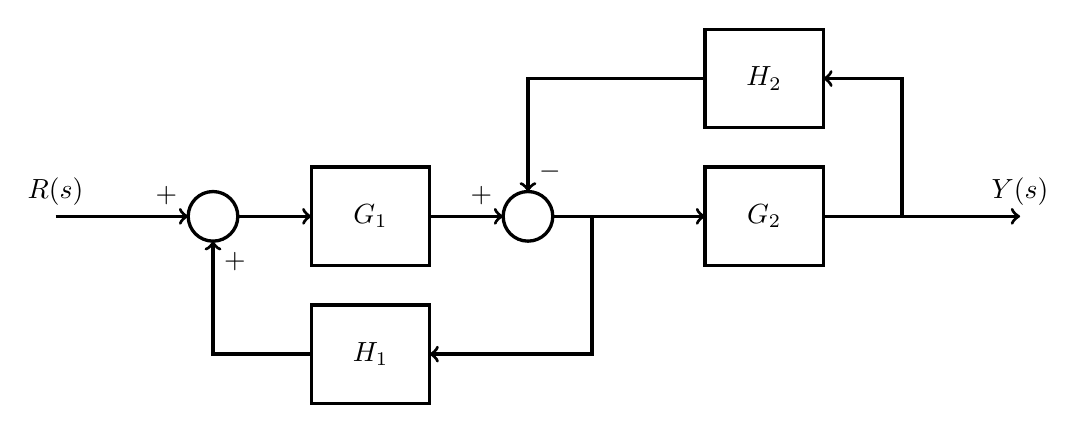
\begin{tikzpicture}[inner sep=0pt,outer sep=0pt,very thick,
sysblock/.style={draw,rectangle,inner sep=2pt,minimum width=1.5cm,minimum height=1.25cm,very thick}]
\draw (-2,0) node[draw,circle] (sum0) {$\rule{0pt}{18pt}$};
\draw (0,0) node[sysblock] (G1) {$G_{1}$};
\draw (2,0) node[draw,circle] (sum1) {$\rule{0pt}{18pt}$};
\draw (5,0) node[sysblock] (G2) {$G_{2}$};
\draw (G2.0) ++(1,0) node[fill=black] (a) {};

\draw (5,1.75) node[sysblock] (H2) {$H_{2}$};
\draw (0,-1.75) node[sysblock] (H1) {$H_{1}$};

\draw[->] (-4,0) node[above=4pt] {$R(s)$} -- (sum0.180) node[above left=4pt] {$+$};
\draw[->] (sum0.0) -- (G1.180);
\draw[->] (G1.0) -- (sum1.180) node[above left=4pt] {$+$};
\draw[->] (sum1.0) -- (G2.180);
\draw (G2.0) -- (a);
\draw[->] (a) -- ++(1.5,0) node[above=4pt] {$Y(s)$};
\draw[->] (a) |- (H2.0);
\draw[->] (sum1.0) ++(0.5,0) |- (H1.0);
\draw[->] (H1.180) -| (sum0.-90) node[below right=4pt] {$+$};
\draw[->] (H2.180) -| (sum1.90) node[above right=4pt] {$-$};

\end{tikzpicture}

\end{center}
